% =====================================================================
%  MeshGraphNets-V / cHI-MGNflow -- paper skeleton
%
%  Build:  pdflatex main && bibtex main && pdflatex main && pdflatex main
%  (or:    latexmk -pdf main.tex)
%
%  Swap \documentclass for the venue style when you pick one; nothing
%  below depends on the article class beyond the packages loaded here.
% =====================================================================
\documentclass[11pt]{article}

\usepackage[utf8]{inputenc}
\usepackage[T1]{fontenc}
\usepackage[margin=1in]{geometry}
\usepackage{amsmath,amssymb}
\usepackage{booktabs}
\usepackage{graphicx}
\usepackage{microtype}
\usepackage[numbers,sort&compress]{natbib}
\usepackage[hidelinks]{hyperref}
\usepackage{placeins}
% Five full-width figures overflow the default float queue, which silently
% pushes them past the bibliography to the end of the document. Loosen the
% per-page limits and bar floats from crossing into the references.
\renewcommand{\topfraction}{0.92}
\renewcommand{\bottomfraction}{0.70}
\renewcommand{\textfraction}{0.06}
\renewcommand{\floatpagefraction}{0.72}
\setcounter{topnumber}{3}
\setcounter{bottomnumber}{2}
\setcounter{totalnumber}{5}
% Generated by audit_data.py; do not transcribe.
\newcommand{\SnapshotDraws}{830}
\newcommand{\SnapshotSuccesses}{830}
\newcommand{\SnapshotFailures}{0}
\newcommand{\TrainDraws}{576}
\newcommand{\TrainDriftFailures}{116}
\newcommand{\TrainDriftPercent}{20.1}
\newcommand{\TrainTopMin}{37.5}
\newcommand{\TrainTopMax}{66.7}
\newcommand{\TrainModesMin}{3}
\newcommand{\TrainModesMax}{5}
\newcommand{\CostExponent}{0.88}



\title{Probabilistic Hierarchical Mesh Graph Networks for\\
       One-to-Many Engineering Simulation}
\author{}
\date{}

\begin{document}
\maketitle

\begin{abstract}
Squared-error mesh simulators target conditional means, which can conceal
variation caused by unobserved physical inputs. We describe two implemented
probabilistic hierarchical mesh simulators: MeshGraphNets-V, with graph-level
latent slots and a conditional flow-matching prior, and cHI-MGNflow, with a
conditional flow on nodal fields. A recorded industrial-warpage sweep reports
best normalised Wasserstein distances of $0.410$ and $0.896$, respectively,
over three parts, together with substantial dispersion deficits. Its original
prediction archives are unavailable in this checkout, so these historical
results are distinguished from reproduced measurements. A Gaussian
counterexample establishes that a flow-matching loss coupled to a trainable
encoder is not a variational KL rate term; it does not establish collapse of
the full training objective. We also construct and audit a shell-compression
dataset with a known withheld spectral imperfection law. A frozen training-tier
snapshot contains $\TrainDraws$ draws over twelve geometries, with
$\TrainModesMin$--$\TrainModesMax$ observed dominant modes per geometry.
However, $\TrainDriftPercent\%$ exceed the specified RMS-drift threshold;
solver completion alone does not certify equilibrium. We document the actual
information boundary, correct thickness handling in the taper solves, and
separate raw finite-time characterisation from filtered exports. No learned
model performance on this shell dataset is claimed.
\end{abstract}

% Introduction and related work. Compile through main.tex.

\section{Introduction}
\label{sec:intro}

\subsection{From point predictions to distributions on meshes}
\label{sec:intro:lineage}

Graph-based learned simulators represent a discretised physical system by
nodes, edges and field values. Graph Network-based Simulators established an
encode--process--decode architecture for particle dynamics, and MeshGraphNets
adapted this approach to simulation meshes~\cite{sanchezgonzalez2020gns,
pfaff2021meshgraphnets}. These models learn point predictions using squared
regression losses. Input noise used to stabilise their rollouts should be
distinguished from an explicit model of the predictive distribution.

Hierarchical processors extend the spatial range of message passing.
MultiScale MeshGraphNets uses information at multiple mesh resolutions, while
BSMS-GNN constructs coarse graphs by bi-stride
pooling~\cite{fortunato2022msmgn,cao2023bsmsgnn}. Operator architectures such
as FNO, GINO and Transolver provide other ways to represent nonlocal
dependencies~\cite{li2021fourier,li2023gino,wu2024transolver}. Architecture
and prediction target are separate choices: using a hierarchy does not by
itself turn a point regressor into a probabilistic simulator. Conversely,
hierarchical probabilistic graph models already exist in weather forecasting
and fluid simulation~\cite{oskarsson2024graphefm,
lino2025diffusiongraphnets,lino2026scaleautoregressive}.

\subsection{What a squared loss elicits}
\label{sec:intro:elicitation}

For finite second moments, minimising expected squared error elicits the
conditional mean. Absolute error elicits a median~\cite{gneiting2007strictly}.
The mean can be useful even when the conditional distribution is broad, but it
does not specify its spread, tails or dependence. In a multimodal problem,
the mean can also lie between physically admissible branches. Thus, an
accurate mean alone does not establish an accurate distribution.

GenCFD examines this distinction for fluid statistics and contrasts
mean-square-trained deterministic models with generative
models~\cite{molinaro2024gencfd}. Related observations about averaging
incompatible futures occur in stochastic video
prediction~\cite{babaeizadeh2018sv2p,denton2018svglp,lee2018savp}.
For engineering meshes, the practical question is whether a surrogate can
generate plausible fields with the correct conditional frequencies, including
the distribution of quantities used in tolerance or reliability calculations.

\subsection{Uncertainty is relative to the observed inputs}
\label{sec:intro:mechanisms}

Let $g$ denote the information supplied to a model. Several different
mechanisms can produce variation across samples, and their interpretation
depends on which variables are included in $g$.

\paragraph{Chaotic dynamics.}
For a deterministic solver conditioned on its complete state and parameters,
the next state is a point mass. Varying initial conditions produces a
trajectory ensemble when those conditions are marginalised out. Partial
observation, coarse resolution and model error can introduce additional
predictive uncertainty; it would therefore be too strong to identify all
weather or turbulent-flow uncertainty with perturbations of a fully observed
state~\cite{price2025gencast,kohl2026acdm}.

\paragraph{A withheld physical variable.}
A deterministic solver can produce different outcomes at the same visible
condition when an imperfection or material field is omitted. The induced law
is $p(y\mid g)$, obtained by integrating over that field. The spread is
irreducible for the stipulated input set, but may decrease if additional
measurements are supplied. This does not, by itself, classify all physical
variability as epistemic uncertainty: data variability and uncertainty about
the predictive model are different notions~\cite{huellermeier2021aleatoric}.
The controlled shell benchmark in this work uses a specified random
imperfection as the withheld variable.

\paragraph{An intrinsically stochastic simulation.}
A kinetic Monte Carlo process can vary even at fixed physical inputs because
of its random draws~\cite{plimpton2009spparks}. Fixing all visible conditions
gives a single distribution to learn. Such a task can quantify uncertainty at
that condition, although it cannot test transfer between conditions. For grain
microstructures, arbitrary grain identifiers also require a representation
that respects relabelling symmetry.

\subsection{What an evaluation can establish}
\label{sec:intro:measurement}

An RMSE of an ensemble mean evaluates the mean. It cannot identify the
ensemble's dispersion or spatial dependence: ensembles with the same mean
receive the same value. A proper score, in contrast, evaluates a predictive
distribution against an observed outcome. One outcome per condition is enough
to form an unbiased observation of the conditional expected score; averaging
over test cases can compare predictive procedures. Repeated outcomes at the
same condition are valuable for estimating that particular conditional law
without pooling assumptions. Their absence limits condition-specific
diagnostics, not the validity of proper scoring~\cite{gneiting2007strictly}.

Finite model ensembles introduce a separate estimation issue. If members are
independent draws from a predictive law, the empirical-distribution CRPS has a
finite-ensemble term that can favour under-dispersed sampling laws. Fair
estimators remove that term under their sampling
assumptions~\cite{ferro2014fair,zamo2018estimation}. The number of reference
outcomes and the number of generated members play different roles and must be
reported separately.

Propriety is an expected-score property, not a guarantee of a correct ranking
in every finite test. Multivariate energy scores may have limited power against
some dependence errors, motivating complementary variogram scores and
diagnostics of spatial structure~\cite{pinson2013discrimination,
scheuerer2015variogram,marcotte2023regions}. Rank histograms and spread
diagnostics help interpret calibration, but cannot establish joint calibration
alone~\cite{hamill2001interpretation}. Section~\ref{sec:protocol} separates
these statistical properties from the metrics actually available in the
reported experiments.

\subsection{Contributions and evidence scope}
\label{sec:intro:contributions}

\begin{enumerate}
  \item \textbf{Two implemented probabilistic mesh simulators.}
    MeshGraphNets-V uses graph-level latent slots across hierarchy levels,
    aggregate-posterior MMD regularisation and a conditional flow-matching
    prior. cHI-MGNflow performs conditional flow matching in field space with
    a hierarchical graph processor. Section~\ref{sec:method} documents the
    implemented objectives and sampling paths. These are related constructions,
    but their training objectives and sampling costs differ, so their
    comparison is not a controlled ablation of stochasticity placement alone.
  \item \textbf{A recorded industrial warpage comparison.}
    The retained research note reports lower normalised scalar Wasserstein
    distance for MeshGraphNets-V and under-dispersion in both model families
    on three evaluated parts. Section~\ref{sec:results:saoi} reports the
    numerical results together with the missing historical configurations and
    raw-output limitation. This evidence concerns a peak-to-valley quantity of
    interest, rather than validation of a joint field distribution.
  \item \textbf{An analytical check of a trainable flow-matching target.}
    A solvable Gaussian example shows that the optimal flow-matching
    regression loss can decrease as the encoded target contracts even when
    the prior matches the target distribution exactly
    (Section~\ref{sec:method:shrink}). This distinguishes the regression loss
    from a variational rate term. It does not prove that the complete
    regularised simulator collapses or explain its observed calibration error.
  \item \textbf{A controlled shell benchmark implementation.}
    The generation plan contains $22$ geometries in four tiers, with a visible
    deterministic imperfection and a separate random component withheld from
    model inputs. Section~\ref{sec:results:buckling} distinguishes planned,
    solved and retained samples and reports dataset characterisation. No
    trained-model result on this benchmark is claimed.
  \item \textbf{An evaluation protocol and a dataset-contract audit.}
    Sections~\ref{sec:protocol} and~\ref{sec:bench} specify fair ensemble
    scoring, diagnostic controls and the information needed to define a
    one-to-many task. The audit identifies observed initial-state variation
    in converted datasets and the failure of raw grain-label regression to
    respect relabelling. Protocol definitions are distinguished from completed
    model evaluations.
\end{enumerate}

\section{Related work}
\label{sec:related}

\subsection{Generative PDE surrogates}
\label{sec:related:diffusion}

Generative PDE models address several targets, including accurate temporal
evolution, stable long rollouts and distributions of physical states.
PDE-Refiner uses denoising refinements to improve the representation of
low-amplitude spatial frequencies in neural PDE solvers~\cite{lippe2023pderefiner}.
Autoregressive conditional diffusion has also been studied for incompressible
and transonic flows and turbulence, with attention to temporal stability and
spectral behaviour~\cite{kohl2026acdm}. GenCFD explicitly targets statistical
fluid quantities~\cite{molinaro2024gencfd}. These objectives should be compared
using their stated observables: pointwise rollout accuracy, stationary
statistics and conditional probabilistic accuracy are related but distinct.

\subsection{Flow matching and coupling choices}
\label{sec:related:fm}

Flow matching trains a time-dependent velocity through regression on a
conditional probability path without integrating the learned ODE during the
basic training objective~\cite{lipman2023flowmatching}. Rectified flows and
stochastic interpolants provide closely related
constructions~\cite{liu2023rectifiedflow,albergo2023buildingflows,
albergo2023interpolants}. The absence of an ODE solve in that objective makes
joint training with an encoder practical, but does not make its full cost
identical to an ordinary regression head; generation still requires numerical
integration unless a different sampler is supplied.

Noise--data coupling is a modelling choice. Minibatch optimal transport can
reduce path length and improve flow-matching efficiency, but a finite-batch
coupling should not be identified with exact population optimal
transport~\cite{tong2024otcfm,pooladian2023multisample}. These literature
variants provide context; the field-flow implementation described here pairs
Gaussian noise with each training target independently.

\subsection{Generative models on unstructured domains}
\label{sec:related:offgrid}

Diffusion Graph Networks and their latent-space variant use multiscale GNNs
to sample statistically developed flows on unstructured meshes, including
varying wing geometries. Their experiments explicitly compare multiscale and
single-scale processors~\cite{lino2025diffusiongraphnets}. The subsequent
scale-autoregressive model generates coarse mesh fields first and finer fields
conditioned on those predictions, using a hierarchy derived from the mesh
and a flow-matching sampler~\cite{lino2026scaleautoregressive}. These are
direct precedents for hierarchical probabilistic mesh generation.

FluidFlow applies conditional flow matching on unstructured
meshes~\cite{ramos2026fluidflow}; the Generative Latent Neural PDE Solver maps
different meshes to a shared structured latent grid before latent flow
matching~\cite{li2025genlatentfm}. The present implementation instead
retains graph processing for its latent conditioning and field generation.
Differences in representation and training factorisation motivate comparison,
but do not establish superiority without matched experiments.

\subsection{Latent-variable surrogates and posterior collapse}
\label{sec:related:vae}

Conditional VAEs learn a recognition distribution that sees the training
target and a prior used when that target is absent~\cite{sohn2015cvae}.
Mismatch between the two distributions can affect generation even when
posterior reconstruction is accurate. Learned conditional priors and
regularisation address this problem without guaranteeing its
elimination~\cite{denton2018svglp,zhao2017infovae}. The MMD-based
aggregate-posterior regulariser used here is motivated by InfoVAE.

Lucas et al.\ analyse posterior collapse through linear VAEs and probabilistic
PCA, showing that the linear ELBO need not introduce additional spurious local
maxima relative to the marginal likelihood~\cite{lucas2019dontblame}. This
does not establish that every nonlinear conditional VAE must collapse or that
KL annealing is ineffective. Similarly, a per-example KL term can constrain
the aggregate posterior as well as information carried by the latent; the
difference from MMD is not the complete absence of aggregate control.
Our Gaussian calculation concerns the scale sensitivity of an additional
flow-matching loss, rather than a general theorem about VAE training.

\subsection{Probabilistic weather forecasting}
\label{sec:related:weather}

WeatherBench~2 includes probabilistic verification alongside deterministic
forecast metrics~\cite{rasp2024weatherbench2}. GenCast learns an ensemble
forecast distribution, while AIFS-CRPS uses an almost-fair CRPS training
objective~\cite{price2025gencast,lang2026aifscrps}. Their verification against
one realised weather trajectory per forecast case is a valid use of proper
scores, with statistical conclusions drawn across cases.

Graph-EFM is especially close architecturally: it samples coarse latent
representations in a hierarchical graph, uses a variational objective, and
adds an unbiased two-member marginal CRPS term during fine-tuning to improve
calibration. It also discusses the tension between marginal scoring and
spatial coherence~\cite{oskarsson2024graphefm}. We therefore do not claim
hierarchical stochasticity, proper-score training or this coherence issue as
new. The implementation studied here uses per-sample engineering meshes,
aggregate MMD regularisation and a flow-matching prior; its empirical evidence
must still be judged independently of those design choices.

\subsection{Operator uncertainty and microstructure}
\label{sec:related:operatoruq}
\label{sec:related:micro}

Bayesian operator methods, deep ensembles and conformal methods address
different aspects of uncertainty~\cite{magnani2022approximatebno,
lakshminarayanan2017deepensembles,ma2024calibrated,psaros2023uqsciml}.
Posterior parameter draws can induce coherent function samples; it would be
incorrect to describe every such method as producing intervals only.
Coverage guarantees and joint generative accuracy should also be distinguished.
Probabilistic neural operators provide another route to distributional
learning using scoring-rule objectives~\cite{bulte2025pno}.

For microstructures, grain identifiers are arbitrary, whereas grain boundaries,
sizes and correlation functions represent physical or morphological
structure~\cite{torquato2002random,plimpton2009spparks}. Generative methods
evaluate such structure using descriptors and statistical
comparisons~\cite{mosser2017porousgan,kench2021slicegan,hoffman2025grainpaint}.
Marginal scores on invariant boundary indicators remain meaningful for local
event probabilities, but do not determine joint morphology. Conversely,
matching a few descriptor moments does not establish equality of field
distributions. These complementary limitations motivate reporting both the
representation being scored and the information it discards.

\subsection{Positioning}
\label{sec:related:gap}

The contribution is a documented implementation and an evidence-bounded
engineering study combining probabilistic graph models with an explicit
hidden-variable benchmark construction. Hierarchical generation, learned
latent priors and proper scoring all have prior art. The recorded industrial
comparison evaluates a scalar response on three parts; the shell study
characterises a generated dataset before model training. Neither establishes
that our hierarchy improves joint field structure, that a persistent latent
has been learned across a rollout, or that calibrated transfer to new shell
families has been achieved. Those claims require additional experiments.



% Benchmark scope and verified local dataset contracts.
% Compile through main.tex.

\section{The benchmark landscape for one-to-many simulation}
\label{sec:bench}

\subsection{Match the dataset to the statistical claim}
\label{sec:bench:criterion}

A distributional task must specify the model-visible condition $g$, the source
of random variation and the outcome being scored. Repeated outcomes at fixed
$g$ permit direct empirical checks of that conditional distribution. They are
not a prerequisite for proper-score evaluation: one outcome at each of many
test conditions can estimate an average predictive score. Such an evaluation
does not, without additional assumptions or observations, resolve calibration
separately at every individual condition~\cite{gneiting2007strictly}.

We therefore distinguish the suitability of a dataset for a specific
hidden-variable experiment from its validity as a probabilistic benchmark.
Table~\ref{tab:landscape} identifies the different claims supported by common
sampling designs. The examples below are a targeted review and an audit of
three local conversions, not an exhaustive census of all available datasets.

\begin{table}[t]
\centering
\small
\caption{Sampling designs and their interpretation. Representation, conditioning
and dependence must be specified separately from the number of samples.}
\label{tab:landscape}
\begin{tabular}{@{}p{0.27\linewidth}p{0.32\linewidth}p{0.32\linewidth}@{}}
\toprule
\textbf{Design} & \textbf{Can evaluate} & \textbf{Main limitation} \\
\midrule
One outcome per condition &
Average proper score across test cases &
Few direct checks of each individual conditional law \\
Replicates at many conditions &
Within-condition distributions and transfer between conditions &
Independent reference samples and a declared condition split are needed \\
Many outcomes at one condition &
A distribution at that fixed condition &
No evidence of transfer between conditions \\
Snapshots from one long run &
A stationary distribution under justified sampling assumptions &
Serial dependence reduces effective sample size \\
Several solver or model variants &
A declared mixture over model choices &
Not automatically physical replicate variability \\
\bottomrule
\end{tabular}
\end{table}

Mesh-based generative fluid benchmarks already contain multiple physical
states for varying geometries~\cite{lino2025diffusiongraphnets,
lino2026scaleautoregressive}. Those states represent statistically developed
flow and need not be independent nonlinear solves with a withheld imperfection.
The distinction motivates our shell construction; it does not justify claiming
that no many-condition, many-outcome mesh benchmark exists.

\subsection{Examples from a public simulation collection}
\label{sec:bench:tier1}

The Well includes several useful seed ensembles, with different conditioning
contracts~\cite{ohana2024well}. Its source documentation must be read at the
level of each subset rather than assuming that every trajectory in the
collection has the same uncertainty mechanism.

\paragraph{Turbulence--gravity--cooling.}
The documented ensemble has $2{,}700$ trajectories: $100$ random seeds for
each of $27$ combinations of initial density, temperature and metallicity.
The public fields are supplied on a structured grid. These counts
describe the simulation design; an evaluation must still declare which initial
fields are exposed to the model and align physical output
times.\footnote{\url{https://polymathic-ai.org/the_well/datasets/turbulence_gravity_cooling/}}

\paragraph{Rayleigh--B\'enard convection.}
The documented design combines five Rayleigh numbers, seven Prandtl numbers,
five initial buoyancy amplitudes and ten noise seeds, giving $1{,}750$
trajectories. If all three non-seed parameters are visible, there are $175$
conditions with ten seeds each. Grouping only by Rayleigh and Prandtl number
instead gives $35$ groups and marginalises over the five buoyancy amplitudes;
these are different prediction tasks. The collection also distinguishes the
original graded grid from a uniformly resampled
version.\footnote{\url{https://polymathic-ai.org/the_well/datasets/rayleigh_benard/}}

\paragraph{Turbulent radiative layer.}
The two-dimensional subset supplies ten seeds for each of nine cooling times.
Our local conversion retains $72$ training trajectories and $18$ inference
trajectories. Its state channels include the velocity perturbation that varies
between seeds; Section~\ref{sec:bench:negative} explains why the visible input
changes the interpretation of this ensemble.

\paragraph{Viscoelastic instability.}
The source describes coexisting dynamical states. A multimodal field law
motivates richer models than a single Gaussian distribution over the output
field, but does not prove that flow matching is necessary: nonlinear latent
decoders and other mixture or generative models can also represent multiple
modes. Any comparison must specify the distribution of initialisations and how
trajectory lengths affect mode
weights.\footnote{\url{https://polymathic-ai.org/the_well/datasets/viscoelastic_instability/}}

None of these counts gives a universal threshold for reliable CRPS or rank
histograms. Precision depends on the target distribution, effect size,
dependence and aggregation rule, as well as the number of generated members
and reference outcomes.

\subsection{Common mismatches between data and claims}
\label{sec:bench:reject}

Several distinctions prevent misleading benchmark conclusions.

\begin{itemize}
  \item \textbf{Visible variability versus hidden variability.}
    Two runs with different material maps or initial velocity fields do not
    share a model-visible condition when those fields are inputs. They can
    still form a valid conditional prediction dataset, but are not replicate
    outcomes at identical inputs.
  \item \textbf{Time samples versus independent realisations.}
    Correlated snapshots may estimate stationary statistics under appropriate
    stationarity and ergodicity assumptions. Treating them as independent
    replicates overstates precision; it does not make the stationary
    distribution itself invalid.
  \item \textbf{An ensemble mean versus a realised field.}
    If the released target is an average over solver runs, its distribution is
    the distribution of that average. Evaluating it does not recover the
    variability of individual runs.
  \item \textbf{Physical variability versus model uncertainty.}
    Alternative constitutive models, solver settings and neural training seeds
    can define useful uncertainty ensembles. Their mixture and weighting must
    be explicit, and should not be labelled independent physical repeats.
\end{itemize}

Mechanical MNIST Crack Path illustrates the first distinction: the original
problem relates microstructural input to mechanically driven
fields~\cite{mohammadzadeh2022crackpath}. Withholding that input changes the
task, but does not automatically make the remaining observed state identical
between cases.

\subsection{A withholding construction and its input boundary}
\label{sec:bench:construction}

The local Mechanical MNIST conversion omits the inclusion field and stores
coordinates, damage and two displacement components on a $256\times256$
regular grid, connected by non-periodic grid edges. It contains $1{,}750$
training cases and $250$ inference cases, each with $20$ stored frames. These
are grid samples of finite-element results, not the original finite-element
mesh. The construction differs from the shell dataset of
Section~\ref{sec:results:buckling}, where the visible and hidden imperfection
components are specified before simulation.

Crucially, the converted crack dataset does \emph{not} have bit-identical
model-visible initial states. A direct comparison of the first two numerically
indexed cases in each HDF5 split finds differences in all three state channels
at the first stored frame. The maximum absolute damage difference is
approximately $0.00881$ in that training pair and $0.0780$ in that inference
pair; both displacement channels differ as well. These counterexamples are
enough to reject identical-input replication, but do not measure how much
information about the final crack is available from that frame.

Thus, $p(y_{\mathrm{future}}\mid \text{stored state})$ and
$p(y_{\mathrm{trajectory}}\mid \text{geometry, loading protocol})$ are
different targets. Omitting the explicit inclusion channel does not remove the
inclusions' mechanical effects from the observed state. Under the current
autoregressive input contract, the stored state is part of the condition.
A genuinely common-state construction would require defining and validating a
common initial input, together with a compatible loading-time convention.
That variant is not supplied by simply dropping the inclusion channel.

The local audit establishes this input-contract limitation. It does not
establish a numerical information-leak floor, the residual conditional
dimension, or a precise branching window. Such results require a reproducible
analysis with specified sample selection, split membership, distance
normalisation and uncertainty estimates. Per-step diagnostics would be
appropriate for locating any branching interval, but are not presented here
as completed measurements.

\subsection{Two candidate slots with different targets}
\label{sec:bench:negative}

\paragraph{A radiative-layer seed ensemble.}
The local radiative-layer files contain nodal arrays of shape
$[8,101,49152]$: three coordinates, density, pressure, two velocity components
and cooling time. Each of the nine cooling times has eight training seeds and
two inference seeds. Comparing two seeds at the same cooling time shows
bit-identical initial density and pressure but different initial velocities.
The model therefore receives at least part of the seed-dependent perturbation.

For a deterministic solver with a complete state, conditioning on that state
removes uncertainty about the next step. This observation does not prove that
the stored fields are a complete Markov state or that a learned predictor has
zero residual uncertainty. It does show why a cross-seed ensemble conditioned
only on cooling time cannot be used directly as the reference conditional law
for a model that also observes the realised velocity field.

The two reference seeds per cooling time are a small sample for estimating a
condition-specific distribution. This reference count does not determine the
number of rank-histogram bins: a histogram for an ensemble of $M$ generated
members has $M+1$ possible ranks, with tie handling specified. Reference count
controls how many rank observations are available, and nodes or timesteps
within a trajectory cannot simply be counted as independent observations.

\paragraph{Grain growth and the meaning of a Brier score.}
The local SPPARKS conversion has $900$ training and $100$ inference samples,
each storing a static $100^3$ grain-identifier array. Numeric grain IDs are
arbitrary labels: a bijective relabelling leaves the partition unchanged
while altering a squared error on the IDs. A separate crop converter provides
a $50^3$ boundary-indicator representation using open faces and a
six-neighbour stencil. The invariant target resolves label symmetry, although
it does not alone specify an adequate morphology metric.

A spatially constant \emph{probability forecast} must not be confused with a
constant generated microstructure. If a boundary event at a node has
probability $p$, the expected Brier score of a forecast probability $q$ is
\begin{equation}
  \mathbb{E}(q-Y)^2 = p(1-p)+(q-p)^2,\qquad Y\sim\operatorname{Bernoulli}(p).
  \label{eq:brier-marginal}
\end{equation}
It is minimised at $q=p$. If a probability is instead estimated as the mean
$\hat q$ of $M$ independent Bernoulli samples with success probability $q$,
independent of the verifying outcome, the expected score gains the term
$q(1-q)/M$. A known probability can therefore outperform the empirical
probability from a finite ensemble sampled from the same law. This is the
finite-ensemble effect addressed by fair scores~\cite{ferro2014fair}, not
evidence against Brier propriety.

If two field distributions have identical probabilities at every node,
summing marginal Brier scores cannot distinguish their spatial dependence.
Scrambling can preserve marginal probabilities while destroying grains.
The appropriate conclusion is to supplement valid marginal probability
scores with joint or morphology-sensitive diagnostics, not to call marginal
scores anti-informative. A proper score applied to a descriptor assesses its
induced distribution; it is strictly informative about the full field only
when the representation and score identify that field law.

At fixed physical settings this is a legitimate distributional task. It can
measure variability at those settings, but supplies no test of conditioning
on varying geometries or process parameters.

\subsection{Design requirements for the shell benchmark}
\label{sec:bench:missing}

The shell construction targets a particular engineering question: how a
withheld imperfection changes the field distribution across known geometries.
Its requirements are (i)~a declared visible-input contract and independently
drawn hidden variables; (ii)~retained mesh connectivity and consistently
defined output fields; (iii)~repeated outcomes and separate condition splits
for within-condition evaluation and transfer; (iv)~documented solver,
convergence and retention criteria; and (v)~engineering quantities of interest
alongside field diagnostics. A deterministic control is useful for detecting
spurious spread, but a matching spread on that control alone cannot certify
calibration.

Sample counts should follow precision or power requirements rather than a
universal cutoff such as $50$ conditions with $50$ members each. Finite
reference self-scores provide a sampling baseline, not a strict lower bound
for every observed score. Likewise, exclusions based on numerical convergence
may change the retained conditional law and must be reported.
Section~\ref{sec:results:buckling} states the implemented construction and
the current evidence for these requirements.



% =====================================================================
%  Methodology -- MeshGraphNets-V and cHI-MGNflow
%  Compile through main.tex.
% =====================================================================

\section{Methodology}
\label{sec:method}

\subsection{Problem statement: predicting a conditional law}
\label{sec:method:problem}

Let $g$ denote everything a learned simulator observes about a scene: the mesh
$(\mathcal{V},\mathcal{E})$, the nodal coordinates, the boundary-condition and
material channels, and any scalar conditions supplied alongside them. Let
$\mathbf{y}\in\mathbb{R}^{N\times F}$ be the field to be predicted at the $N$
mesh nodes. The deterministic simulator lineage---GNS, MeshGraphNets, and the
hierarchical variants including HI-MGN---learns a map $\hat{\mathbf{y}} =
f_\theta(g)$ under a pointwise regression loss,
\begin{equation}
  \mathcal{L}_{\mathrm{MSE}}(\theta)
  = \mathbb{E}_{(g,\mathbf{y})}\bigl\|f_\theta(g)-\mathbf{y}\bigr\|_2^2 ,
  \label{eq:mse}
\end{equation}
whose population minimiser is the conditional mean
$f^\star(g)=\mathbb{E}[\mathbf{y}\mid g]$.

The conditional mean is optimal for squared-error point prediction, but does
not specify uncertainty when $p(\mathbf{y}\mid g)$ is broad. Write the data-generating
process as
\begin{equation}
  \mathbf{y} = \mathcal{S}(g,\boldsymbol{\xi}),
  \qquad \boldsymbol{\xi}\sim p(\boldsymbol{\xi}\mid g),
  \label{eq:generative}
\end{equation}
where $\mathcal{S}$ is the physical solver and $\boldsymbol{\xi}$ is a latent
variable that governs the response but is \emph{not} part of $g$: an
unmeasured geometric imperfection, a process-to-process manufacturing
deviation, a microstructural realisation. The quantity of engineering interest
is then the conditional law
\begin{equation}
  p(\mathbf{y}\mid g)
  = \int p\bigl(\mathbf{y}\mid g,\boldsymbol{\xi}\bigr)\,
         p(\boldsymbol{\xi}\mid g)\,\mathrm{d}\boldsymbol{\xi},
  \label{eq:marginal}
\end{equation}
and a model trained under \eqref{eq:mse} returns a single point estimate.
When \eqref{eq:marginal} is multimodal, as can occur in buckling mode
selection, the conditional mean need not lie in its support: averaging
physically realisable states can produce a field that is itself unrealizable. Tolerance
analysis, yield prediction and reliability assessment all require the width and
shape of \eqref{eq:marginal}, not its centroid.

We therefore ask a model to emit \emph{samples} and compare the generated and
reference ensembles. Section~\ref{sec:protocol} distinguishes the historical
SAOI scalar-distance metric from the implemented buckling energy score. The
two mesh-native constructions below place stochasticity in a graph latent or
directly in the field. This section describes the current implementation;
the historical SAOI results in Section~\ref{sec:results} are not a validation
of every subsequently added option.

\subsection{Shared backbone}
\label{sec:method:backbone}

Both models inherit the encode--process--decode structure of MeshGraphNets and
the hierarchical processor of HI-MGN. Node and edge features are embedded by
MLPs into latent vectors $\mathbf{v}_i$ and $\mathbf{e}_{ij}$, and each message
passing (MP) block performs
\begin{align}
  \mathbf{e}_{ij}' &= f_E\bigl(\mathbf{e}_{ij},\,\mathbf{v}_i,\,\mathbf{v}_j\bigr),
  \label{eq:mp-edge}\\
  \mathbf{v}_i'    &= f_V\Bigl(\mathbf{v}_i,\;
                        \textstyle\sum_{j\in\mathcal{N}(i)}\mathbf{e}_{ij}'\Bigr),
  \label{eq:mp-node}
\end{align}
with residual connections, after which a decoder MLP reads the nodal output.
The receptive field expands by at most one mesh hop per block; communicating
between arbitrary nodes through this path alone requires depth at least the
graph diameter. HI-MGN replaces the flat stack with a multiscale processor.
Farthest-point sampling chooses seeds and multi-source breadth-first search
assigns nodes to their nearest seed in graph distance. Coarse edges are
induced by fine edges crossing cluster boundaries. In
\texttt{voronoi\_seedmean} mode, features are mean-pooled while coarse
positions use the seed nodes. MP blocks run at each level, and a learned
graph interpolation network reconstructs fine-resolution features on the way
back up. For example, the current SAOI arm-1 configurations specify two
coarsening levels with $1000$ and $100$ requested coarse nodes, hidden width
$128$, and a $4,6,8,6,4$ MP schedule. Other arms vary capacity or conditioning.
Sharing this hierarchy does not make the full models identical: posterior,
prior, input dimensions, modulation and training objectives also differ.

A note on the input contract. The \texttt{cond\_var} channels following the
state rows in \texttt{nodal\_data} are
\emph{conditions}: quantities the model reads but never predicts (process
settings, known boundary values). They enter $\mathbf{x}$ alongside the state,
positional and node-type features, receive their own normalisation statistics,
and are retained as known inputs during an autoregressive rollout. For the
static $T=1$ contract, the state input is zero and the target is the absolute
output field; temporal data instead use the next-step increment as target.
The conditions are part of $g$; the latent $\boldsymbol{\xi}$ of
\eqref{eq:generative} is, by construction, not.

\subsection{MeshGraphNets-V: a latent-variable simulator}
\label{sec:method:mgnv}

MeshGraphNets-V (MGN-V) uses a conditional variational-encoder architecture
with an aggregate-posterior MMD objective, rather than a KL-based ELBO. A graph-level latent
$\mathbf{z}\in\mathbb{R}^{K\times d}$ carries the sample-to-sample spread while
the processor carries what geometry and boundary conditions determine. The
latent is organised as $K=L+1$ \emph{slots}, one per hierarchy level plus the
fine level, each of width $d$; the current SAOI configuration uses
$K=3$, $d=16$, i.e.\ $48$ latent coordinates in total. These are graph-level
slots injected at different levels, not a latent vector at every coarse node.

\paragraph{Posterior.}
A GNN encoder sees the normalised target and edge features and, when
\texttt{vae\_graph\_aware=True} as in the current SAOI configurations, also
the normalised input-node features. It runs message passing and
pools to a single graph vector by attention, from which all slots are emitted:
\begin{equation}
  q_\phi(\mathbf{z}\mid \mathbf{y},g)
  = \mathcal{N}\bigl(\boldsymbol{\mu}_\phi(\mathbf{y},g),\,
                     \operatorname{diag}\boldsymbol{\sigma}^2_\phi(\mathbf{y},g)\bigr).
  \label{eq:posterior}
\end{equation}

\paragraph{Decoder.}
The HI-MGN simulator itself is the decoder. Each hierarchy level receives its
corresponding slot at every MP block. The implementation supports a linear
concatenation fuser and AdaLN-Zero modulation; the current SAOI configurations
select AdaLN-Zero. The posterior variance is diagonal conditional on its
inputs, although mixing over targets can induce dependence between slots.

\paragraph{Conditional prior.}
At inference the target is unavailable. With the learned conditional prior
enabled, $\mathbf{z}$ is drawn from $p_\psi(\mathbf{z}\mid g)$. Its default family is conditional
flow matching in latent space: a velocity network transports
$\mathcal{N}(\mathbf{0},\mathbf{I})$ onto the posterior cloud for that graph,
conditioned on a pooled graph embedding, and is integrated by a Heun or Euler
ODE solver. All slots are flattened jointly, so cross-slot dependence is
learned rather than assumed factorised. The implemented path retains endpoint
noise with standard deviation $10^{-4}$ in the prior's working coordinates.
An optional frozen-prior training phase freezes the encoder and decoder,
standardises posterior latents using training-set moments, and fits only the
prior; sampling undoes that affine standardisation. A legacy
graph-conditioned Gaussian mixture and standard-normal latent sampling are
also available. They are distinct inference choices, not equivalent priors.

\paragraph{Objective.}
For joint training with the flow-matching prior, the current loss is
\begin{equation}
  \mathcal{L}_{\text{MGN-V}}
  = \alpha_{\mathrm{recon}}\,\mathcal{L}_{\mathrm{recon}}
  + \lambda_{\mathrm{MMD}}\,\mathcal{L}_{\mathrm{MMD}}
  + \beta_{\mathrm{aux}}\,\mathcal{L}_{\mathrm{aux}}
  + w_{\mathrm{prior}}\,\mathcal{L}_{\mathrm{FM}},
  \label{eq:mgnv-loss}
\end{equation}
where $\mathcal{L}_{\mathrm{recon}}$ is the channel-weighted, node-averaged
posterior reconstruction error in normalised target coordinates (MSE in the
current SAOI configurations; Huber is also supported).
$\mathcal{L}_{\mathrm{MMD}}$ averages a multi-bandwidth RBF MMD squared over
slots, comparing minibatch posterior samples with independent
$\mathcal{N}(0,I)$ samples. It uses the biased V-statistic, including diagonal
kernel terms, with fixed or detached median-based bandwidths. This is
aggregate-posterior regularisation in the InfoVAE sense
\citep{zhao2017infovae}; it does not match each conditional posterior to the
learned $p_\psi(\mathbf{z}\mid g)$, or constrain the joint cross-slot law.
$\mathcal{L}_{\mathrm{aux}}$ is the graph-averaged squared error between
predicted and target peak-to-valley values of a selected normalised output
channel. For $T=1$ this is the field statistic; for temporal data it is the
increment statistic. It encourages reconstruction of that statistic without
guaranteeing calibrated spread or a mutual-information lower bound.
$\mathcal{L}_{\mathrm{FM}}$ is the flow-matching
loss that fits the conditional prior to a \emph{fresh} posterior sample drawn
each step. A switch $g_{\mathrm{enc}}\in[0,1]$ scales the gradient that
$\mathcal{L}_{\mathrm{FM}}$ sends back through the encoder; at
$g_{\mathrm{enc}}=0$ the prior chases a detached posterior, and at
$g_{\mathrm{enc}}=1$ the encoder also receives the velocity-regression
gradient through the path point and target.
Section~\ref{sec:method:shrink} shows why that second coupling is not the
variational rate term it resembles.

\subsection{cHI-MGNflow: flow matching in field space}
\label{sec:method:flow}

cHI-MGNflow places the stochasticity at the output instead of in a bottleneck.
It learns a conditional flow directly on the $N\times F$ field. Let
$\mathbf{y}_1$ be the normalised target and
$\mathbf{y}_0\sim\mathcal{N}(\mathbf{0},\mathbf{I})$ an independent Gaussian
source drawn at every node and channel. With $s=1-\sigma_{\min}$ the
conditional path and its velocity are, with the implemented
$\sigma_{\min}=10^{-4}$,
\begin{align}
  \mathbf{y}_t &= (1-s\,t)\,\mathbf{y}_0 + t\,\mathbf{y}_1,
  \label{eq:flow-path}\\
  \mathbf{u}   &= \mathbf{y}_1 - s\,\mathbf{y}_0 ,
  \label{eq:flow-target}
\end{align}
and the network regresses the velocity,
\begin{equation}
  \widehat{\mathcal{L}}_{\mathrm{flow}}
  = \frac{\sum_b w(t_b)\sum_{i=1}^{N_b}\sum_f a_f
    \bigl(v_\theta(\mathbf{y}_{t_b},t_b,g_b)_{if}-u_{bif}\bigr)^2}
    {\sum_b N_b w(t_b)} ,
  \label{eq:flow-loss}
\end{equation}
where $a_f$ are nonnegative channel weights normalised to sum to one, and
$b$ indexes graphs in a collated training minibatch. The implementation normalises by the
realised sum of node-time weights (with a numerical denominator floor), not
by an expectation over $t$. Without time weighting, $w(t)=1$. The flow time
$t$ is drawn \emph{per graph}, not per node: the velocity field
is a function of the whole field state, so mixing times inside one graph would
depart from the stated whole-field path. The hierarchical
processor is traversed once per velocity evaluation, with $t$ entering through
AdaLN modulation and the noisy field entering alongside the conditions.

The default \texttt{flow\_head=v} predicts velocity directly. An optional
data-prediction weighting, called \texttt{x0} in the configuration, uses
$w(t)=(1-st)^2$. The per-node loss identity is exact:
\begin{equation}
  \hat{\mathbf{y}}_1 = s\,\mathbf{y}_t + (1-s\,t)\,\hat{\mathbf{u}}
  \quad\Longrightarrow\quad
  \bigl\|\hat{\mathbf{y}}_1-\mathbf{y}_1\bigr\|^2
  = (1-s\,t)^2\bigl\|\hat{\mathbf{u}}-\mathbf{u}\bigr\|^2 ,
  \label{eq:x0-equiv}
\end{equation}
The batch normalisation in \eqref{eq:flow-loss} still applies. Separately,
the current code supports \texttt{flow\_head=x}, whose network output is a
clean-field estimate $h_\theta$ and whose returned velocity is
\begin{equation}
 v_\theta = \frac{h_\theta-s\mathbf{y}_t}
 {\max(1-st,\varepsilon_{\mathrm{head}})} .
 \label{eq:flow-x-head}
\end{equation}
The default floor is $\varepsilon_{\mathrm{head}}=0.05$. This conversion
equals the unfloored path identity only where $1-st\geq
\varepsilon_{\mathrm{head}}$. Without this floor, the gain reaches $10^4$ at
$t=1$; it is finite at the implemented positive $\sigma_{\min}$ and becomes
singular only in the zero-noise limit. Thus output-head choice and time-loss
weighting are separate options.

Time sampling can be uniform or logit-normal, with an optional probability
of pinning a graph to $t=0$. At that endpoint, independence of
$\mathbf{y}_0$ and $\mathbf{y}_1$ gives the population regression optimum
$v^*(\mathbf{y}_0,0,g)=\mathbb{E}[\mathbf{y}_1\mid g]-s\mathbf{y}_0$.
The implemented one-evaluation readout is
$\mathbf{y}_0+v_\theta(\mathbf{y}_0,0,g)$, which at this optimum equals
$\mathbb{E}[\mathbf{y}_1\mid g]+\sigma_{\min}\mathbf{y}_0$. Its error also
depends on how well the trained network fits $t=0$.

Sampling integrates the learned ODE from $t=0$ to $t=1$ with Euler or Heun,
holding the graph hierarchy fixed. Even with the exact marginal velocity
and exact integration, the stated path ends at
$\mathbf{y}_1+\sigma_{\min}\mathbf{y}_0$, so its target law is the
Gaussian-smoothed data law. A finite network and finite integration budget
introduce additional approximation error.

\subsection{A contraction mechanism in trainable-target flow matching}
\label{sec:method:shrink}

A tempting reading of \eqref{eq:mgnv-loss} is that opening the encoder gradient
($g_{\mathrm{enc}}=1$) turns $\mathcal{L}_{\mathrm{FM}}$ into the
$D_{\mathrm{KL}}\bigl(q(\mathbf{z}\mid\mathbf{y},g)\,\|\,p(\mathbf{z}\mid
g)\bigr)$ rate term of a conditional VAE, making \eqref{eq:mgnv-loss} an ELBO.
It does not. A Gaussian counterexample exhibits the difference.

The flow-matching theorem \citep{lipman2023flowmatching} equates the gradients of the conditional and marginal
velocity-regression objectives \emph{with respect to the velocity model's
parameters, for a fixed target distribution}. It says nothing about gradients
with respect to parameters that \emph{move} the target. A VAE rate term
contains the posterior entropy and vanishes whenever $q=p$. The optimised
flow-matching MSE need not vanish when its endpoint distribution is matched.

The consequence is quantitative. Consider the scalar Gaussian instance
$Z_0\sim\mathcal{N}(0,1)$, $Z_1\sim\mathcal{N}(0,a^2)$ independent, with the
linear path $Z_t=(1-t)Z_0+tZ_1$ and velocity target $U=Z_1-Z_0$. Here $a$
plays the role of the trainable posterior scale, with $a>0$. This example
sets $\sigma_{\min}=0$ to give a simple closed form. Since $(U,Z_t)$ is jointly
Gaussian, the optimal regressor is the conditional expectation and its
irreducible loss is the conditional variance,
\begin{equation}
  \operatorname{Var}\bigl(U \mid Z_t\bigr)
  = (1+a^2) - \frac{\bigl(a^2t-(1-t)\bigr)^2}{(1-t)^2+a^2t^2}
  = \frac{a^2}{(1-t)^2+a^2t^2}.
  \label{eq:cond-var}
\end{equation}
Integrating over a uniform time schedule gives the loss floor attained by a
\emph{perfectly} trained velocity model,
\begin{equation}
  \int_0^1 \operatorname{Var}\bigl(U\mid Z_t\bigr)\,\mathrm{d}t
  = \int_0^1 \frac{a^2}{(1-t)^2+a^2t^2}\,\mathrm{d}t
  = \frac{\pi a}{2}.
  \label{eq:floor}
\end{equation}
The floor is \emph{linear in $a$}. Meanwhile a prior that matches the target
exactly has $D_{\mathrm{KL}}=0$ for every $a$. So the optimised flow-matching
objective can always be decreased by shrinking the target distribution, even
though the density-matching problem it is supposed to represent is already
solved perfectly at every scale. In this Gaussian example, allowing the
encoder scale to optimise the best-achievable FM loss therefore creates
contraction pressure even with unlimited prior capacity. For the implemented
positive endpoint noise, the corresponding variance is
$a^2/[(1-st)^2+a^2t^2]$; its derivative with respect to $a$ is
$2a(1-st)^2/[(1-st)^2+a^2t^2]^2>0$, so the scale incentive remains in this
example. This calculation concerns the FM term alone, without reconstruction,
MMD, variance floors or latent standardisation.

The counterexample shows that a trainable-target FM loss is not generally a
VAE rate term. It does not establish the net effect of the coupling in a
nonlinear, jointly trained model, nor rule out an empirical benefit. The
historical SAOI note reports a small observed contrast for this factor
(Section~\ref{sec:results}); the incomplete, unreplicated sweep cannot prove
that the causal effect is zero or identify the cause of under-dispersion.

% =====================================================================
%  Evaluation protocol -- proper scores for mesh-valued ensembles
%  Compile through main.tex.
% =====================================================================

\section{Evaluation protocol}
\label{sec:protocol}

A distributional claim must specify the predicted quantity, the reference
sample and the estimator. The historical SAOI comparison uses distances and
diagnostics of scalar peak-to-valley values. The buckling scoring module
implements a fair energy score on spectral descriptors. These are different
evaluation scopes; neither a scalar statistic nor a phase-discarding descriptor
identifies the full displacement-field law.

\subsection{Proper scores and the ensemble-size correction}
\label{sec:protocol:proper}

Let $\{\mathbf{x}_i\}_{i=1}^{m}$ be the model's ensemble for a scene and
$\mathbf{y}$ an observation. Evaluating the energy score of the empirical
ensemble distribution gives
\begin{equation}
  \mathrm{ES}\bigl(\{\mathbf{x}_i\},\mathbf{y}\bigr)
  = \frac{1}{m}\sum_{i=1}^{m}\bigl\|\mathbf{x}_i-\mathbf{y}\bigr\|_2
  \;-\;\frac{1}{2m^2}\sum_{i=1}^{m}\sum_{j=1}^{m}
       \bigl\|\mathbf{x}_i-\mathbf{x}_j\bigr\|_2
  \label{eq:es}
\end{equation}
The population energy score is strictly proper for multivariate distributions
with finite first moment, and its univariate specialisation is the continuous
ranked probability score (CRPS) \citep{gneiting2007strictly}. If the ensemble
members are independent draws from a model distribution, then
\eqref{eq:es}, viewed as an estimator of that distribution's score, has
upward bias $\mathbb{E}\|X-X'\|/(2m)$. The buckling module therefore defaults
to the \emph{fair} estimator for $m\geq2$, replacing $m^2$ by $m(m-1)$
\citep{ferro2014fair}:
\begin{equation}
  \widetilde{\mathrm{ES}}
  = \frac{1}{m}\sum_{i}\bigl\|\mathbf{x}_i-\mathbf{y}\bigr\|_2
  \;-\;\frac{1}{2m(m-1)}\sum_{i}\sum_{j}\bigl\|\mathbf{x}_i-\mathbf{x}_j\bigr\|_2 .
  \label{eq:fair-es}
\end{equation}
This is unbiased over independent model draws for the population score
against a fixed observation. Fairness is not guaranteed for arbitrarily
dependent ensemble members. For a singleton deterministic forecast, the
implementation returns its distance to the observation. For independent
standard-normal forecasts and observations, the expected fair CRPS is
$1/\sqrt{\pi}$, while the expected empirical-ensemble CRPS is
$(1+1/m)/\sqrt{\pi}$. This analytic example isolates the ensemble-size bias
without relying on a particular Monte-Carlo realisation.

\subsection{Reference self-score and mean-only baseline}
\label{sec:protocol:baselines}

The energy score inherits the units and scaling of its descriptor. Even at
the true population distribution $Q$, its expected value is generally
positive: $\mathbb{E}_{Y\sim Q}\mathrm{ES}(Q,Y)=
\tfrac12\mathbb{E}_{Y,Y'\sim Q}\|Y-Y'\|$. This reflects intrinsic spread,
not merely finite reference-sample error. The buckling report provides two
empirical anchors for interpreting this value.

The quantity stored as \texttt{self\_floor} is a \emph{reference self-score}:
the implementation randomly splits the reference sample into two disjoint
halves, scores one half against every member of the other with the fair
estimator, and averages over $20$ splits (default random seed $0$). It
estimates the true-distribution score but is not a lower bound on any finite
realisation of a model's score. Repeated splits of the same sample are also
not independent replication. The \emph{mean-only reference} scores the sample's
own mean as a singleton forecast against that same sample. It is a descriptive
oracle baseline using evaluation outcomes, not a separately trained regressor.
The implemented skill transformation is
\begin{equation}
  \mathrm{SS} = \frac{\mathrm{ES}_{\mathrm{ref}}-\mathrm{ES}}
                     {\mathrm{ES}_{\mathrm{ref}}-\mathrm{ES}_{\mathrm{floor}}}
  \label{eq:skill}
\end{equation}
It equals $1$ at the estimated self-score and $0$ at the mean-only reference.
It can exceed $1$ or be negative; these anchors do not bound finite-sample
scores. A non-finite or nearly zero denominator produces an undefined skill.
Its uncertainty depends on the finite reference and generated ensembles.

\subsection{Dispersion is a separate question from location}
\label{sec:protocol:dispersion}

A score alone does not attribute error to ensemble location or width. The
current SAOI ranking script, \texttt{configs/campaigns/rank\_arms.py}, reads
saved scalar peak-to-valley samples and reports the following diagnostics.

The \emph{dispersion ratio} $\mathrm{sd}(\text{gen})/\mathrm{sd}(\text{ref})$
has population target $1$; below $1$ the generated scalar values have less
empirical spread. Both standard deviations use divisor $n$, as in
\texttt{numpy.std} with its default \texttt{ddof=0}. The \emph{bias}
$\bigl(\overline{\text{gen}}-\overline{\text{ref}}\bigr)/\mathrm{sd}(\text{ref})$
has target $0$; its magnitude measures a mean offset in reference standard
deviations. Neither diagnostic certifies distributional calibration.

The empirical rank statistic is
$r_j=m^{-1}\sum_i\mathbb{1}\{x_i<y_j\}$, using strict less-than comparison
without random tie-breaking. The script reports its distance from a uniform
CDF and the fraction with $r_j\leq0.02$ or $r_j\geq0.98$. With continuous
i.i.d.\ draws from a calibrated distribution, ranks are uniform on the
$m+1$ discrete rank values; the corresponding tail mass approaches $0.04$
for large $m$. Finite ensemble size, ties and reuse of one forecast ensemble
affect the diagnostic, so the reported KS value is descriptive, not an
independent-observation significance test. U-shaped or domed histograms can
suggest under- or over-dispersion, but bias and heterogeneous conditional
errors can also change their shape. Rank diagnostics and dispersion ratios
are complementary, not statistically independent tests.

The buckling module instead reports \texttt{spread\_ratio}, computed as
$\sqrt{\operatorname{mean}_f\operatorname{var}_{\mathrm{gen}}(X_f)}$
(sample variance with divisor $m-1$) divided by the RMS distance of reference
descriptors from the generated mean. Its denominator includes mean bias;
this is a spread-to-RMSE diagnostic, not the SAOI standard-deviation ratio.
For independent calibrated draws and $m\geq2$, the ratio of its population
second-moment scales is $\sqrt{m/(m+1)}$, which the module reports as an
i.i.d.\ moment reference. This is not the expected value of the finite-sample
ratio itself.

\subsection{Phase-discarding buckling descriptors}
\label{sec:protocol:symmetry}

The buckling energy-score implementation maps each radial-displacement field,
expressed in units of shell thickness, to circumferential Fourier magnitudes.
It takes complete even-indexed axial rows, subtracts each row's mean, retains
harmonics $1$ through $40$ by default, and concatenates the unnormalised FFT
magnitudes without per-draw amplitude normalisation. Thus it retains spectral
amplitude information while discarding the axisymmetric component, phase and
higher harmonics.

Fourier magnitudes are invariant to cyclic shifts of each sampled ring, but
are not a complete quotient by a single physical rotation: different
relative phases between harmonics or axial stations can give the same
descriptor. Nor does a deterministic imperfection in a fixed mesh establish
an exactly $SO(2)$-invariant conditional law. The score is strictly proper for
the \emph{descriptor distribution}, not for the full field or its buckle
location. Raw-field proper scoring remains valid when rotational variation
is part of the prediction target; discarding phase is an evaluation choice,
not a requirement of proper scoring. When mode labels are supplied, the
module additionally reports total variation and Jensen--Shannon divergence
between their empirical histograms.

\subsection{Scalar distances and repeated conditional observations}
\label{sec:protocol:crps-caveat}

CRPS remains proper with one observation per condition: propriety is an
expectation over verifying observations, not a requirement for repeated
outcomes at an identical condition. Limited data can nevertheless make
conditional calibration and model comparisons uncertain. Repeated
realisations at the same condition permit direct estimation of conditional
spread, which is why the historical SAOI design used $125$ outcomes per
evaluated part. These are finite reference samples, not the exact conditional
law.

The SAOI note ranks models by a normalised scalar Wasserstein distance,
not by CRPS or field-space energy score. The current ranking script
approximates the one-dimensional quantile integral at $512$ midpoint
probabilities using interpolated empirical quantiles:
\begin{equation}
 \widehat W_1/\widehat\sigma_{\mathrm{ref}}
 = \frac{1}{512\widehat\sigma_{\mathrm{ref}}}
   \sum_{k=1}^{512}\left|
    \widehat F_{\mathrm{gen}}^{-1}\!\left(\frac{k-1/2}{512}\right)
   -\widehat F_{\mathrm{ref}}^{-1}\!\left(\frac{k-1/2}{512}\right)\right|.
 \label{eq:saoi-w1}
\end{equation}
It averages per-part values to rank arms. This is an empirical distribution
distance with sampling and quadrature error; the fair-score correction in
\eqref{eq:fair-es} does not apply to it. The historical configurations and
raw score arrays are unavailable in the current checkout, so the historical
table in Section~\ref{sec:results:saoi} is attributed to the research note
rather than presented as a newly reproduced evaluation.

\section{Numerical results}
\label{sec:results}

We distinguish a historical industrial experiment recorded in a research note
from a reproduced characterisation of the shell solver outputs. The former
motivates the distributional task; the latter checks the implemented data
construction before a learned model is evaluated on it.

\subsection{Injection-moulded warpage (SAOI)}
\label{sec:results:saoi}

\subsubsection{Task and evidence boundary}
The local September 2026 SAOI research note records three held-out parts, each
with 125 reference realisations and 2000 generated draws. Its quantity of
interest is final-step peak-to-valley $z$ displacement,
$\max_i u_{z,i}-\min_i u_{z,i}$. The reported Wasserstein and mean errors are
normalised by the reference quantity's standard deviation; the dispersion
ratio is $\mathrm{sd}_{\mathrm{gen}}/\mathrm{sd}_{\mathrm{ref}}$.

These numbers are reproduced from the note's tables, not recomputed from
predictions: the original SAOI HDF5 files, prediction archives and complete
historical run configurations are absent from the source tree audited for this
draft. The current \texttt{SAOI\_sweep} profiles describe replacement full
factorial experiments and must not be used as provenance for this older
fractional factorial. The historical interpretation is therefore conditional
on the note's stated data grouping and preprocessing. In particular, 125
realisations estimate a conditional law; they do not specify it exactly.

\subsubsection{Recorded comparison}
The note describes eight planned arms per model at 1000 epochs, with four
factors in a $2^{4-1}$ fractional factorial. For MGN-V these were latent
conditioning, encoder-gradient coupling, capacity and MMD weight; for
cHI-MGNflow they were batch size, flow-time sampling, capacity and learning
rate. One MGN-V arm failed during training, leaving seven recorded results.
No replicated training-seed uncertainty or convergence study accompanies the
table. Shared architectural components do not make this a controlled ablation
of stochasticity placement alone: the two objectives, capacities and tuning
factors also differ.

\begin{table}[tbp]
\centering
\caption{Historical SAOI note, mean over three parts. These are recorded
summary values, not a reproduction from raw predictions. Lower $W_1/\mathrm{sd}$
is better; dispersion ratio one matches the reference width but does not by
itself establish calibration.}
\label{tab:saoi-best}
\begin{tabular}{llccc}
\toprule
model & arm & $W_1/\mathrm{sd}$ & $|\Delta\mathrm{mean}|/\mathrm{sd}$ & dispersion ratio \\
\midrule
MeshGraphNets-V & 7 & 0.410 & 0.218 & 0.475 \\
MeshGraphNets-V & 3 & 0.434 & 0.176 & 0.526 \\
cHI-MGNflow & 1 & 0.896 & 0.724 & 0.475 \\
\bottomrule
\end{tabular}
\end{table}

The ratio of the two best recorded distances is $0.896/0.410\approx2.2$.
Across the available arms, MGN-V spans $0.410$--$0.510$ and cHI-MGNflow spans
$0.896$--$1.604$. These observed ranges do not overlap; this is not a confidence
interval or a claim about untested hyperparameters or additional geometries.

\begin{figure}[tbp]
\centering
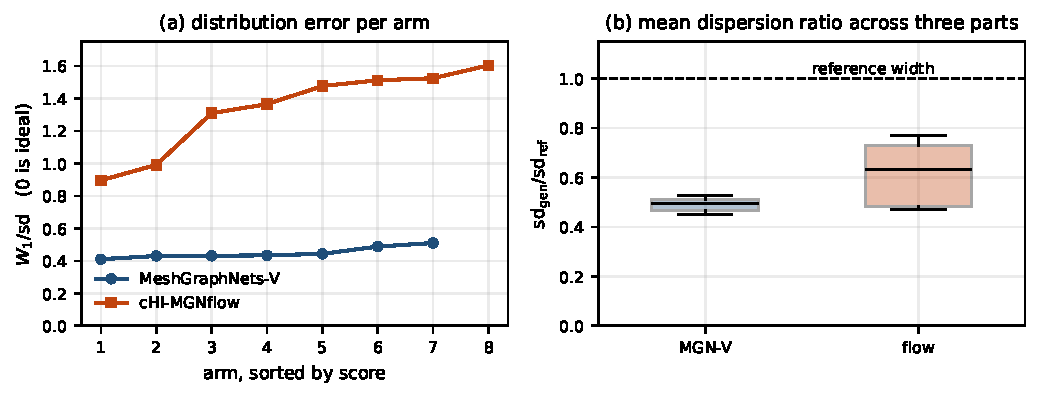
\includegraphics[width=\linewidth]{figures/saoi_ranking.pdf}
\caption{Recorded SAOI arm summaries. Each point or boxplot entry is an arm's
mean over three parts; variation across arms is not training-seed uncertainty.}
\label{fig:saoi-ranking}
\end{figure}

\subsubsection{Location and dispersion}
The note reports particularly large location errors for cHI-MGNflow on
SM-L345U-MAIN: arm 1 has normalised $W_1=1.425$ and signed mean error $1.408$;
arm 7 has $3.659$ and $3.641$. A location error is itself a distributional
calibration defect. Opposite bias signs on different parts do not rule out a
normalisation or preprocessing error; diagnosing the cause requires the
missing raw inputs, predictions and normalisers.

The largest mean dispersion ratio in the table is $0.769$ for cHI-MGNflow;
MGN-V's largest is $0.526$. The former also has per-part ratios above one on
SM-L345U-MAIN, so the average deficit must not be described as uniform across
all parts. Matching neither location nor width is a concern for tolerance
analysis, but failure probabilities depend on thresholds and tail shape and
were not measured here.

\begin{figure}[tbp]
\centering
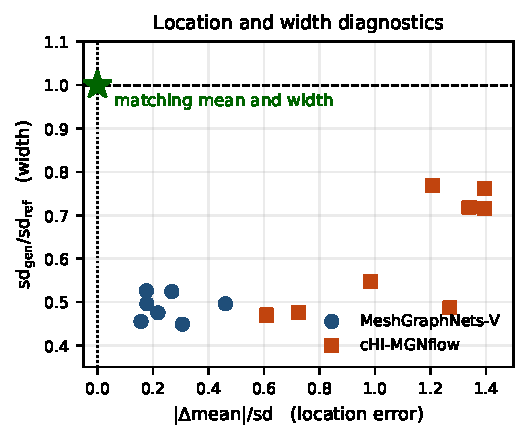
\includegraphics[width=0.60\linewidth]{figures/failure_modes.pdf}
\caption{Recorded location and width diagnostics, averaged over the three
parts for each arm. Agreement in these two moments would still leave the
distribution's shape and field dependence untested.}
\label{fig:failure-modes}
\end{figure}

\subsubsection{Factor effects and limitations}
\label{sec:results:limits}
The note's cHI-MGNflow factor contrasts are $0.333$ for flow-time sampling
(uniform lower), $0.288$ for batch size (16 lower than 32), $0.083$ for
learning rate and $0.074$ for capacity. At fixed epochs, batch size also
changes the number of optimiser updates. The largest MGN-V contrast is
$0.054$ for capacity; its encoder-gradient contrast is only $0.001$.
The missing arm breaks the balanced design, and neither sweep has replication
to distinguish these contrasts from training variability or aliased effects.
Consequently the small encoder-gradient contrast does not prove a null effect
or rule out an intervention, and the flow-time contrast does not establish a
general rule about mesh fields versus images.

The Gaussian example in Section~\ref{sec:method:shrink} distinguishes two
objectives mathematically. It does not diagnose the cause of these historical
dispersion deficits. Reproducing the SAOI evaluation requires restoring the
original data, model states, run configurations and prediction archives.

\subsection{Shell benchmark with a known withheld variable}
\label{sec:results:buckling}

\begin{figure}[tbp]
\centering
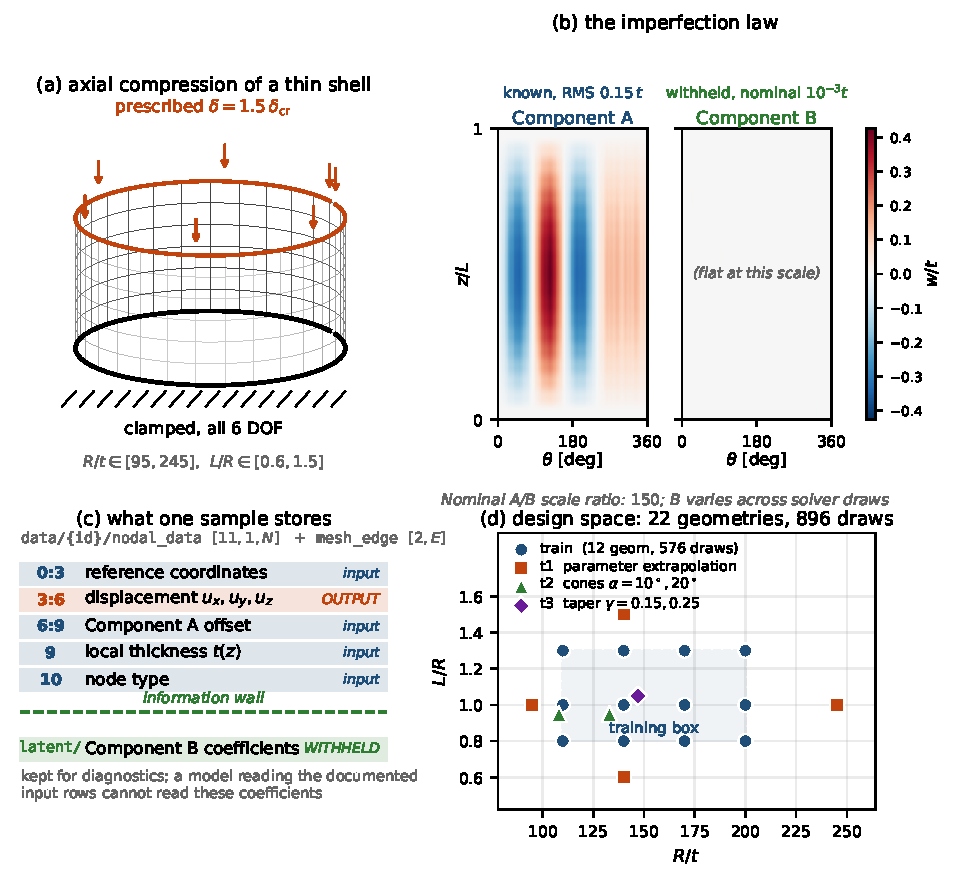
\includegraphics[width=\linewidth]{figures/dataset_overview.pdf}
\caption{Implemented construction: axial compression; deterministic and
withheld imperfection components on a common colour scale; the static HDF5
contract; and the planned geometry tiers. The setup mesh is generated at a
coarser resolution for illustration. Of eleven stored rows, eight provide
visible geometry/conditions and three hold targets that static loaders zero
in the state input. The nominal A-to-B scale ratio is 150; B's realised RMS
varies. Coincident design markers are offset for legibility.}
\label{fig:dataset}
\end{figure}

\subsubsection{Geometry, loading and imperfection law}
The implemented solver uses analytic S8R meshes, reference radius $R=1$,
elastic modulus $E=1$, Poisson ratio $0.3$ and mass density $1$ in consistent
normalised units. The base is clamped; the top is fixed transversely and in
rotation and is driven axially. The static step reaches
$0.70\,\delta_{\mathrm{cr}}$, followed by implicit dynamics over time 8 to
$1.5\,\delta_{\mathrm{cr}}$ and a hold over time 40. These are fixed solver
protocol parameters. The final displacement is a finite-time response;
equilibrium must be checked separately.

The mesh rule targets three quadratic elements per nominal half-wavelength
$1.728\sqrt{Rt}$, with integer rounding and a circumferential resonance
avoidance adjustment. This is approximately six nodal intervals per
half-wavelength, not a mesh-convergence study. The twelve training geometries
have 5311--15190 nodes. The line $0.86\sqrt{R/t}$ is the implementation's
empirical mode reference, used also to guard the signature harmonics; it is
not an independently derived classical buckling prediction.

Component A is a deterministic sum of circumferential harmonics with a
$\sin(\pi z/L)$ envelope. Harmonics within three wavenumbers of the empirical
reference are removed, and the sampled nodal RMS is normalised to $0.15t$.
It is identical across draws of a geometry. Component B uses a Mat\'ern-shaped
spectral density with nominal scale $10^{-3}t$, length parameter
$0.70\sqrt{Rt}$ and smoothness parameter $1.5$. The implementation draws
independent uniform Fourier phases with fixed spectral amplitudes and takes
the real part of the sum over a rectangular frequency truncation. It is not
an exact Gaussian Mat\'ern field or an exactly normalised RMS realisation.
The axial field is defined on a padded length $2L$ and cropped to the shell.
Archived coefficients are float32, so later evaluation avoids interpolation
but does not reproduce the original float64 field bit-for-bit.

The nominal scale ratio $0.15/10^{-3}=150$ expresses how small B is relative
to the supplied signature. Its consequences are measured on the solver
outputs, rather than asserting that B is the only possible numerical source
of branch selection. The non-axisymmetric A and the discrete mesh also
preclude an assertion of exact rotational symmetry of the conditional law.

\subsubsection{Plan and model-visible contract}
\begin{table}[tbp]
\centering
\caption{Planned dataset. Counts precede quality filtering. Tiers t1--t3 are
held out from model fitting. Remaining inside the training interval of local
$R/t$ reduces one extrapolation confound; it does not isolate every geometric
or discretisation effect.}
\label{tab:buckling-tiers}
\begin{tabular}{llrrl}
\toprule
tier & family & geometries & draws & local $R/t$ \\
\midrule
train & cylinders & 12 & 576 & 110--200 \\
t1 & cylinders & 4 & 128 & 95, 140, 245 \\
t2 & cones, $10^\circ$/$20^\circ$ & 4 & 128 & approximately 115--191 \\
t3 & sinusoidal thickness variation & 2 & 64 & approximately 112--140 \\
\bottomrule
\end{tabular}
\end{table}

The shared HDF5 layout is $[11,1,N]$ nodal data plus directed mesh edges.
Rows 0--2 are perfect-shell coordinates; rows 3--5 are displacements measured
from the imperfect starting surface; rows 6--8 are the known A offset;
row 9 explicitly supplies local thickness $t(z)$ in the reference length
units; row 10 is the boundary node type. Thus \texttt{input\_var=3},
\texttt{output\_var=3}, and \texttt{cond\_var=5}. This is a static
condition-to-terminal-field task with one stored frame. The state input is
zeroed by the static loader; copying its stored target rows into the input
would invalidate the withholding construction. The B coefficients and
outcome diagnostics are stored separately under \texttt{latent/} and in
metadata, and must not become model features.

An audit corrected the taper deck: the original writer supplied uniform
thickness even when the plan specified $t(z)$. The corrected writer supplies
nodal thickness, and the generator and exporter reject legacy taper archives
without matching versioned solve settings. The export also requires an
explicit plan and tier selection, since the training loaders do not enforce
tier metadata. A random within-file split is not a geometry-holdout test.

\subsubsection{Reproduced characterisation}
The immutable source snapshot captured on 13 September 2026 at 07:32 KST
contains $\SnapshotDraws$ returned solver-success records and
$\SnapshotFailures$ returned failure records. It includes the complete
training tier, $\TrainDraws$ draws over twelve geometries, and 254
non-training draws. It is an explicitly dated snapshot, not the current
generator progress. Input hashes and per-geometry measurements accompany
this draft; all displacement, radial-field and stored-spectrum relationships
were recomputed from the archives.

\begin{figure}[tbp]
\centering
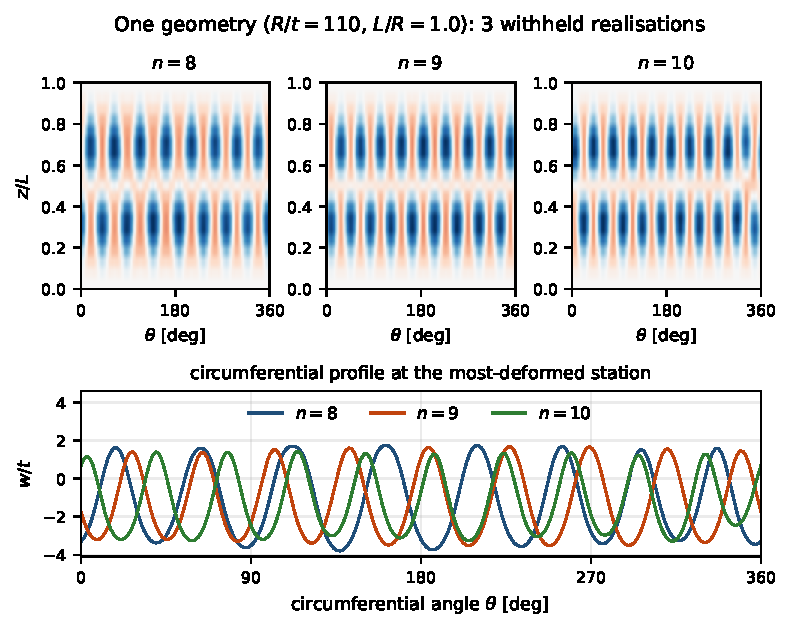
\includegraphics[width=0.82\linewidth]{figures/buckling_fields.pdf}
\caption{Three selected draws at $R/t=110$, $L/R=1.0$, one per observed
dominant mode. Top: radial displacement divided by nominal thickness, with
an individual colour range per panel. Bottom: circumferential profiles at
the respective maximum-response axial stations. Selection illustrates modes,
not their probabilities; the frequency distributions are shown separately.}
\label{fig:buckling-fields}
\end{figure}

\begin{figure}[tbp]
\centering
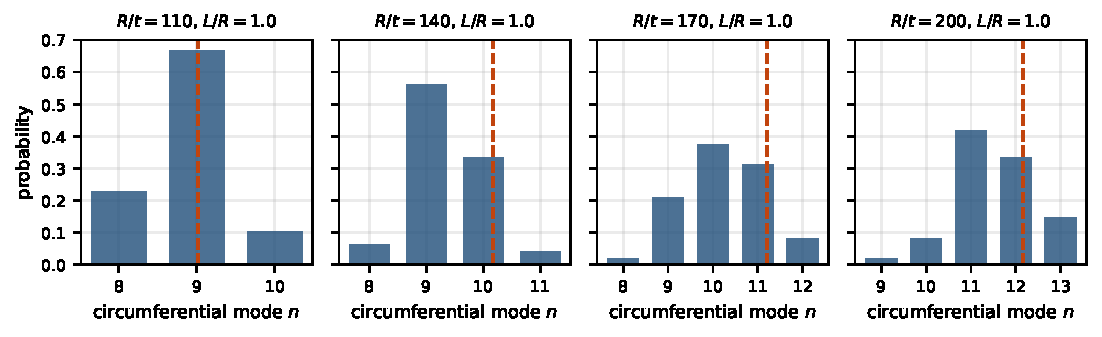
\includegraphics[width=\linewidth]{figures/buckling_modes.pdf}
\caption{Unfiltered finite-time outcomes at fixed $L/R=1.0$, 48 draws per
geometry. Dashed lines show the empirical reference $0.86\sqrt{R/t}$.
All panels use the frozen training-tier records.}
\label{fig:buckling-modes}
\end{figure}

Across the twelve training geometries, the dominant-mode label takes
$\TrainModesMin$--$\TrainModesMax$ distinct values and the largest mode share
is $\TrainTopMin$--$\TrainTopMax\%$. The mean observed mode lies below the
empirical reference by 1.6--13.1\%. These are measured finite-time label
frequencies; no eigenvalue-spectrum or equilibrium study here establishes
the mechanism behind their changes.

The recorded drift is the range of radial RMS divided by its mean over the
last third of saved displacement blocks. Of the training draws,
$\TrainDriftFailures/\TrainDraws$ ($\TrainDriftPercent\%$) exceed 0.15.
For $L/R=0.8$, 1.0 and 1.3, the exceedance counts are respectively 0, 22 and
94 out of 192. Constant RMS can coexist with a changing field shape, so even
a low value is not a force-residual or equilibrium certificate. The raw
characterisation retains these draws and reports their drift; the default
quality-filtered HDF5 export excludes them and therefore represents a
selected subset of the original imperfection law. Both counts and rejection
reasons must accompany an export to avoid hiding this selection effect.

For a dimensionally consistent cross-geometry diagnostic, we also compare
the first 40 nonzero modes of each axially averaged magnitude spectrum after
unit-$L^2$ normalisation. The unbiased sample energy distances over the 66
unordered training-geometry pairs range from 0.030 to 1.050. This descriptor
discards amplitude, phase and axial arrangement and is distinct from the
per-station descriptor in Section~\ref{sec:protocol}. Positive empirical
distances without a sampling-uncertainty analysis do not prove statistical
separation of every pair. The full stored field contains information omitted
by either this spectrum or its argmax label; their relative usefulness for a
learned model remains to be tested.

\subsubsection{Status and remaining validation}
The contribution demonstrated here is an implemented data construction and
an audit of its outputs. No trained-model comparison, calibrated shell
surrogate, autoregressive shell rollout or persistent-latent benefit is
reported. Corrected taper runs are tracked separately from the invalid
uniform-thickness results. Stronger equilibrium claims require displacement,
force and energy convergence checks and sensitivity to the loading/settling
protocol and mesh; larger, quality-filtered samples alone cannot supply that
evidence.

\section{Conclusions}
\label{sec:conclusion}

MeshGraphNets-V and cHI-MGNflow implement two probabilistic extensions of a
hierarchical mesh simulator: graph-level latent slots with a conditional prior,
and a conditional field-space flow. Their implemented training objectives are
reconstruction/MMD/prior matching and flow matching, respectively. Proper
scores used for validation or evaluation must not be described as their
training objectives without specifying the actual training path.

The historical SAOI note reports lower peak-to-valley distribution error for
MGN-V across the recorded arms, together with substantial location and width
defects. Those results concern three parts, not population-wide performance.
The missing original predictions and run configurations prevent an independent
reproduction of that experiment, and the incomplete, unreplicated sweep cannot
establish a null effect of encoder-gradient coupling. Our Gaussian
counterexample establishes only that the flow-matching loss is not the KL
rate term of a variational objective; it does not predict collapse of the
complete implemented loss.

The shell construction makes the withheld imperfection law explicit. A
reproduced snapshot contains $\TrainDraws$ training draws over twelve
geometries, with $\TrainModesMin$--$\TrainModesMax$ observed dominant modes
and top-mode shares of $\TrainTopMin$--$\TrainTopMax\%$. Its audit also
exposes material limitations: $\TrainDriftPercent\%$ exceed the RMS-drift
threshold, and a low RMS drift alone does not establish equilibrium. We
corrected the taper thickness supplied to the solver and added checks against
reusing invalid legacy results or mixing inference tiers into training.
Quality filtering and the raw finite-time ensemble describe different
sampling populations and are reported separately.

No learned-model result on this shell dataset is yet established. Completing
equilibrium and discretisation validation, restoring the historical SAOI
experiment artifacts, and evaluating both full fields and engineering
quantities with calibrated uncertainty are the remaining steps toward a
reproducible comparison. The present implementation and measurements support
the construction and its stated limits, rather than a claim that either
architecture has solved distributional engineering simulation.


\appendix
\section{Benchmark generation cost}
\label{app:cost}

Table~\ref{tab:cost} recomputes elapsed time from the frozen training-tier
records, with 48 draws per geometry and 19 concurrent single-threaded solver
jobs. The recorded time covers imperfection construction, solver execution and
output handling. It is elapsed time under this concurrency, not measured CPU
time or an isolated-solver benchmark. The Batdorf parameter is
$Z=(L^2/Rt)\sqrt{1-\nu^2}$.

\begin{table}[tbp]
\centering
\caption{Frozen training-tier generation timings. No cached zero-time records
enter these summaries. Geometry is given as $(R/t,L/R)$.}
\label{tab:cost}
\begin{tabular}{lrrrr}
\toprule
geometry & $Z$ & nodes & mean [s] & range [s] \\
\midrule
% Generated from the frozen, hashed training-tier draws.
$110$, $0.8$ & 67 & 5311 & 1043 & 1023--1054 \\
$140$, $0.8$ & 85 & 6450 & 1319 & 1290--1342 \\
$170$, $0.8$ & 104 & 7952 & 1791 & 1757--1816 \\
$110$, $1$ & 105 & 6328 & 1362 & 1353--1385 \\
$200$, $0.8$ & 122 & 9610 & 2269 & 2230--2301 \\
$140$, $1$ & 134 & 8385 & 2028 & 1958--2115 \\
$170$, $1$ & 162 & 10082 & 2516 & 2489--2542 \\
$110$, $1.3$ & 177 & 8362 & 2079 & 2064--2097 \\
$200$, $1$ & 191 & 11935 & 3078 & 3020--3112 \\
$140$, $1.3$ & 226 & 10707 & 2924 & 2884--3021 \\
$170$, $1.3$ & 274 & 12638 & 3560 & 3531--3606 \\
$200$, $1.3$ & 322 & 15190 & 4613 & 4524--4793 \\

\bottomrule
\end{tabular}
\end{table}

An ordinary least-squares fit of log mean elapsed time against log $Z$ gives
exponent $\CostExponent$ over these twelve geometries. Node count and geometry
co-vary with $Z$ in this design; the fit neither isolates their effects nor
predicts a new mesh, solver protocol or hardware platform without validation.
The within-geometry ranges describe the measured seeds and do not imply
deterministic runtimes.

\section{Implementation configuration and reproducibility}
\label{app:config}

The checked-in SAOI profiles are later experiments, not the original sweep
reported in Section~\ref{sec:results:saoi}. Both current arm-1 profiles use two
coarse levels (1000 and 100 nodes), a $4,6,8,6,4$ message-passing schedule,
hidden width 128, four cached hierarchy variants and loss weights
$(0.1,0.1,1)$. They differ in more than stochasticity placement: the current
MGN-V arm uses 1000 training epochs and input-noise scale 0.01, while the
current cHI-MGNflow arm uses 2000 epochs and input-noise scale zero.
These values describe executable profiles, not recovered historical settings.
Architecture options and their objectives are specified in
Section~\ref{sec:method}.

The manuscript's buckling measurements are generated by
\texttt{paper/audit\_data.py} from a frozen JSON snapshot and SHA-256-identified
draw archives. This recomputes mode labels, spectra, radial displacements,
drift counts and timing tables; it does not rerun the nonlinear solves or
recover deleted force/energy histories. Plot scripts consume the same frozen
record list. The source/PDF checker verifies included files, references,
citations, figure existence and a build manifest; scientific evidence remains
bounded by the audits described in the text.

For the corrected taper runs, the archive records the solver settings,
including nodal-thickness schema, to prevent reuse of the original
uniform-thickness solves. Export requires explicit plan and tier selection,
checks the declared boundary displacement and field arrays, and records all
rejections. Each model's loader must still be configured for the documented
static information boundary. A validation/test split of draws from a known
training geometry evaluates new realisations; a held-out geometry tier
evaluates geometric transfer. These are different tasks.


\FloatBarrier
\bibliographystyle{plainnat}
\bibliography{references}

\end{document}
